%%%%%%%%%%%%%%%%%%%%%%%%%%%%%%%%%%%%%%%%%%  不使用 authblk 包制作标题  %%%%%%%%%%%%%%%%%%%%%%%%%%%%%%%%%%%%%%%%%%%%%%
%-------------------------------PPT Title-------------------------------------
\title{化学-化工知识图谱的建设与应用}
%-----------------------------------------------------------------------------
%----------------------------Author & Date------------------------------------

%\author[\textrm{Jun\_Jiang}]{姜\;\;骏\inst{}} %[]{} (optional, use only with lots of authors)
%% - Give the names in the same order as the appear in the paper.
%% - Use the \inst{?} command only if the authors have different
%%   affiliation.
\institute[BCC]{\inst{}%
%\institute[Gain~Strong]{\inst{}%
\vskip -20pt 北京市计算中心}
%\vskip -20pt {\large 格致斯创~科技}}
\date[\today] % (optional, should be abbreviation of conference name)
{%	{\fontsize{6.2pt}{4.2pt}\selectfont{\textcolor{blue}{E-mail:~}\url{jiangjun@bcc.ac.cn}}}
\vskip 45 pt {\fontsize{8.2pt}{6.2pt}\selectfont{%清华大学\;\;物理系% 报告地点
	\vskip 5 pt \textrm{2023.10.14}}}
}

%% - Either use conference name or its abbreviation
%% - Not really information to the audience, more for people (including
%%   yourself) who are reading the slides onlin%%   yourself) who are reading the slides onlin%%   yourself) who are reading the slides onlineee
%%%%%%%%%%%%%%%%%%%%%%%%%%%%%%%%%%%%%%%%%%%%%%%%%%%%%%%%%%%%%%%%%%%%%%%%%%%%%%%%%%%%%%%%%%%%%%%%%%%%%%%%%%%%%%%%%%%%%

\subject{}
% This is only inserted into the PDF information catalog. Can be left
% out.
%\maketitle
\frame
{
%	\frametitle{\fontsize{9.5pt}{5.2pt}\selectfont{\textcolor{orange}{“高通量并发式材料计算算法与软件”年度检查}}}
\titlepage
}
%-----------------------------------------------------------------------------

%------------------------------------------------------------------------------列出全文 outline ---------------------------------------------------------------------------------
%\section*{}
%\frame[allowframebreaks]
%{
%  \frametitle{Outline}
%%  \frametitle{\textcolor{mycolor}{\secname}}
%  \tableofcontents%[current,currentsection,currentsubsection]
%}
%%在每个section之前列出全部Outline
%%类似的在每个subsection之前列出全部Outline是\AtBeginSubsection[]
%\AtBeginSection[]
%{
%  \frame<handout:0>%[allowframebreaks]
%  {
%    \frametitle{Outline}
%%全部Outline中,本部分加亮
%    \tableofcontents[current,currentsection]
%  }
%}

%-----------------------------------------------PPT main Body------------------------------------------------------------------------------------
\small
%\section{\rm{VASP~}软件中\rm{PAW~}计算的实现}
%\frame
%
%	\frametitle{\textrm{VASP}计算的特色}
%	相比于与普通的第一原理计算软件,\textrm{VASP}很好地平衡了计算效率和精度的问题,总的来说,\textrm{VASP}主要通过这几个特色保证了计算的高效能
%	\begin{itemize}
%	     \item 迭代与优化算法的多样性\\
%		     本质上电荷密度迭代 \textrm{\&\&} 体系总能量优化是相同的优化问题,采用了类似的算法\upcite{CMS6-15_1996,PRB54-11169_1996}:\\
%			\textcolor{blue}{\textrm{Pseudo-Newton、Conjugate-Gradient、Broyden~mix、damping-factor、RMM-DIIS}}
%	     \item 尽可能采用局域基(原子轨道基)函数:~\\
%		     \textcolor{blue}{\textrm{LREAL}}=\textcolor{red}{\textrm{.TRUE.}}\\
%			优化的投影函数也尽可能在实空间表示
%	     \item \textrm{PAW}原子数据集:\textcolor{blue}{优异的赝势}\upcite{PRB59-1758_1999}
%	\end{itemize}
%}
\frame
{
	\frametitle{数据、信息与知识}
\begin{figure}[h!]
\centering
\vskip -10pt
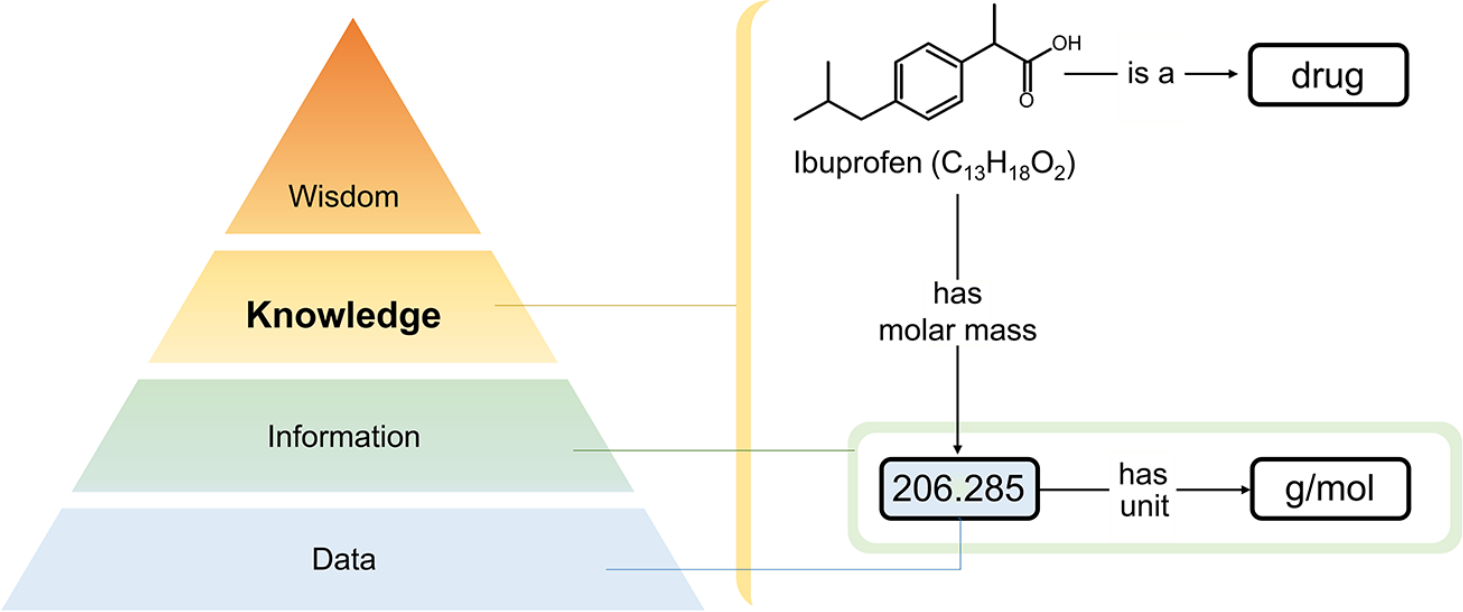
\includegraphics[height=1.75in,width=4.00in,viewport=0 0 1490 615,clip]{DIKW_pyramid-illustrating-data_information-knowledge.png}
\caption{\tiny\textrm{Schematic representation of the DIKW pyramid illustrating the meaning of data, inforamation, and knowledge in the chemical context.\cite{ACR56-128_2023}}}%(与文献\cite{EPJB33-47_2003}图1对比)
\label{Fig:Knowledge-based_system}
\end{figure}
\textcolor{magenta}{知识}\textrm{(Knowledge)}:\\
哲学学科——诸如认知论和方法论——中的核心主题
}

\frame
{
	\frametitle{知识图谱}
	\textcolor{blue}{知识图谱}~\textrm{(Knowledge Graph)}:
	\begin{itemize}
		\item 一种用于组织、表示和存储知识的图形化数据结构形式
		\item \textcolor{purple}{目的}:~使计算机能够更好地认知、理解和推理知识\\
			仿照人类对于知识的认知、理解方式\\
			将实体\textrm{(Entities)}、关系\textrm{(Relationship)}和属性\textrm{(Attributes)}以图形的形式呈现出来,
		\item \textcolor{purple}{技术底层}:~基于语义网\textrm{(Semantic Web)}技术\\
			以\textrm{Web}数据的内容(即语义)为核心,用机器能够理解和处理的方式链接起来的海量分布式数据库
	\end{itemize}
%	知识图谱得益于\textrm{Web}的发展(主要的是数据层面),有着来源于\textrm{KR}、\textrm{NLP}、\textrm{Web}、\textrm{AI}多个方面的基因
\begin{figure}[h!]
\centering
\vskip -8pt
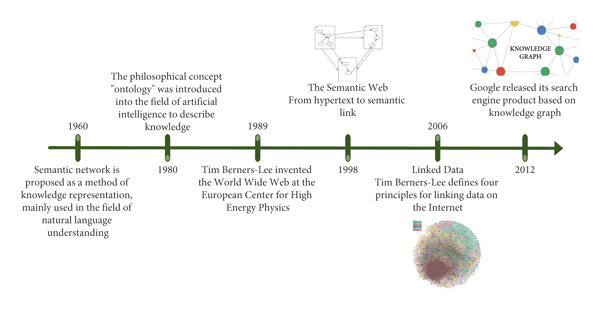
\includegraphics[height=1.00in,width=2.50in,viewport=0 0 160 75,clip]{Development-history-of-the-knowledge-graph.jpg}
\caption{\tiny\textrm{Schematic representation of the development history of the Knowledge Graph.}}%(与文献\cite{EPJB33-47_2003}图1对比)
\label{Fig:Knowledge-history}
\end{figure}
}

\frame
{
	\frametitle{知识图谱的要素}
知识图谱以图形结构的方式,通常使用节点(实体)和连线/边(关系)的形式表示知识\\
这种结构使得知识点之间的关联关系更加清晰和可视化

主要的关键词为:
\begin{itemize}
	\item 实体\textrm{(Entities)}:~知识图谱中的实体是指具体的事物、概念、人物、地点等,每个实体都有一个唯一的标识符。例如,在一个化学知识图谱中,分子、合成体、密度等都可以是实体。
	\item 关系\textrm{(Relationships)}:~实体之间的关系表示不同实体之间的连接或互动。这些关系可以是有向的或无向的,用于描述实体之间的各种联系,如” 具有”、” 属于”、”值为” 等。
	\item 属性\textrm{(Attributes)}:~实体可以有一些描述性的属性,这些属性是与实体相关的额外信息。例如,一个分子实体可以有属性包括分子量、化合价、密度等。
\end{itemize}
}

%------------------------------------------------------------------------Reference----------------------------------------------------------------------------------------------
		\frame[allowframebreaks]
{
\begin{thebibliography}{99}
\frametitle{主要参考文献}
{\tiny
\bibitem{ACR56-128_2023}\textrm{A. Kondinski, J. Bai, S. Mosbach, J. Akroyd, and M. Kraft. \textit{Acc. Chem. Res.}, \textbf{56} (2023), 128}
}
\end{thebibliography}
%\nocite*{}
}
